La figura de este problema representa un circuito constituido por tres lámparas $L_1$, $L_2$ y $L_3$, alimentado por una batería de fem $\epsilon$ = 32 V y resistencia interna $r$ = 0.50 $\Omega$. Al cerrar el circuito con el interruptor $S$, se observa que en las lámparas se disipan las siguientes potencias: $P_1$ = 30 W, $P_2$ = 45 W y $P_3$ = 45 W, respectivamente. Sabiendo que en cada 10 segundos la batería transforma 1280 J. de su energía interna en energía eléctrica de las cargas, calcule la corriente $i_3$ que pasa por $L_3$, y el valor de la resistencia, $R_3$, de tal foco.
\begin{figure}[h!]
  \centering
  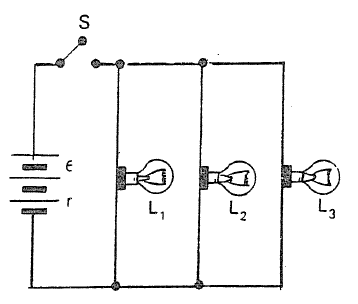
\includegraphics[scale=0.6]{enunciados/figuras/fig_alvarenga_p1007_19.png}
  \caption{Alvarenfa p1007 - Problema 19}
\end{figure}